\chapter{Problema}

No contexto de simulações de fenômenos aeroacústicos usando Lattice Boltzmann, normalmente o campo de pressão ao longo do espaço é referente ao campo próximo e, por limitações de recursos computacionais, criar uma malha grande o suficiente para englobar o campo distante inviabiliza de forma integral a simulação. O presente problema a ser estudado e analisado diz respeito a um sólido quadrado que está sofrendo a influência de um escoamento de velocidade horizontal. O presente sistema é retratado de acordo com a figura \ref{fig1}.

\begin{figure}[h!]
    \centering
    \hspace{-1.cm}
    \label{fig1}
    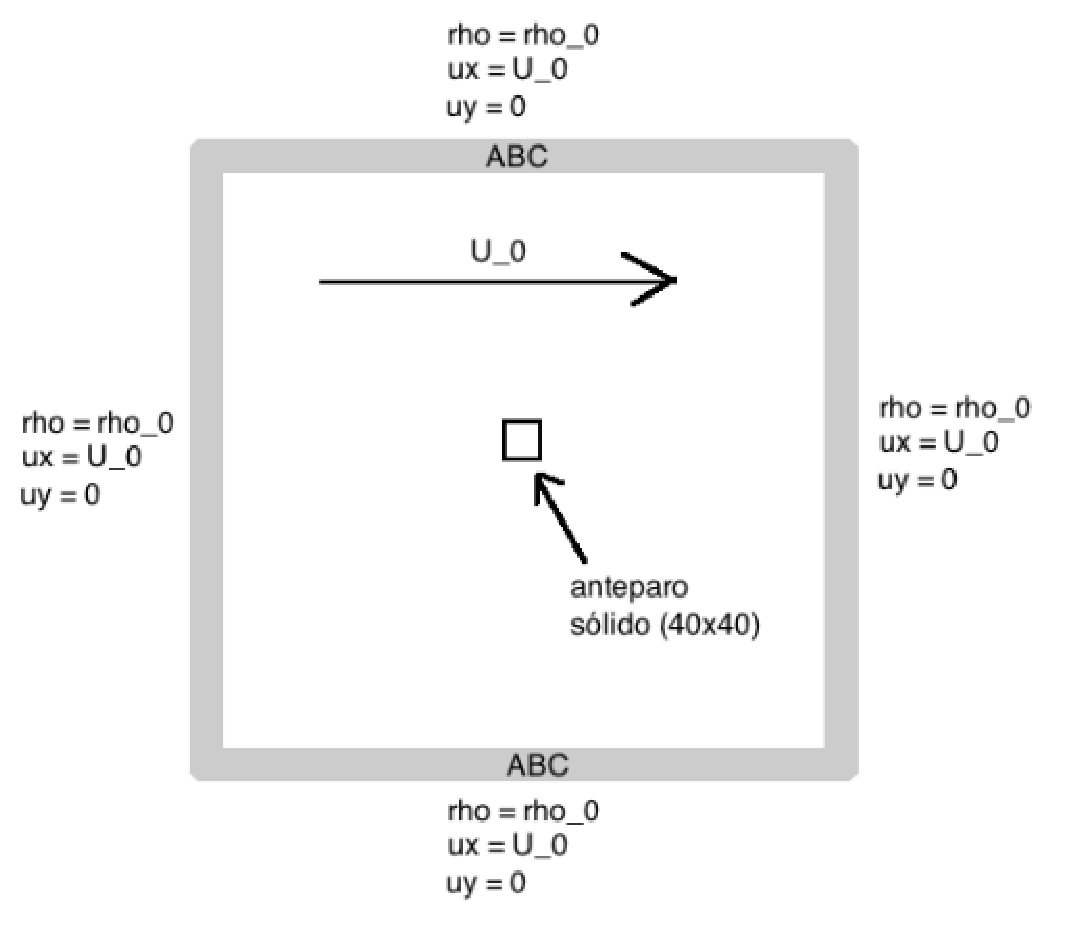
\includegraphics[width=0.5\textwidth]{../figuras/l5_1.eps}
    \caption{Esquemático do problema.}
\end{figure}

Diante do contexto exposto, propõe-se submeter esse sistema a um escomento de velocides Mach = 0.07 e 0.1. Além disso a superfície de FW-H será variada de 1 célula até 100 células de Lattice e análise da diretividade em campo distante há 15 metros da fonte.

\chapter{Solução e Implementação}

Para mitigar o problema da captação do campo distante dado as limitações computacionais, há a proposta de \cite{lockard} que utiliza da superfície de Ffowcs Williams and Hawkings para extrapolar resultados para o campo distante usando a composição do espectro de frequências do campo acústico próximo. Para a aplicação dessa técnica é preciso delimitar uma região para essa superfície e aplicar a equação da figura \ref{fig2}.

\begin{figure}[h!]
    \centering
    \hspace{-1.cm}
    \label{fig2}
    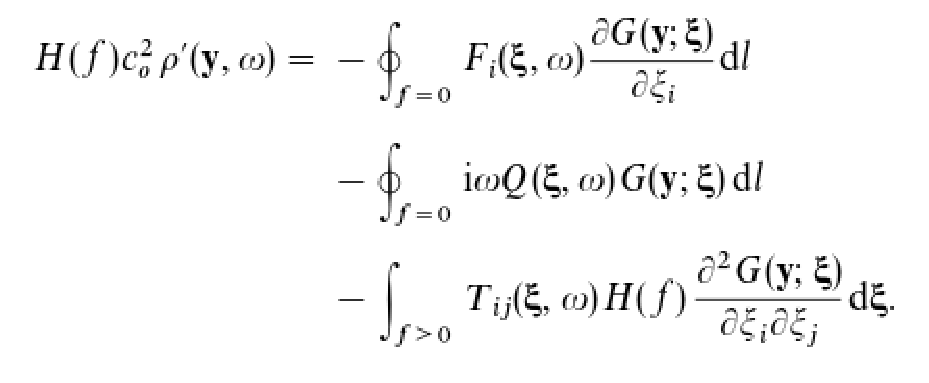
\includegraphics[width=0.7\textwidth]{../figuras/l5_2.eps}
    \caption{Equação da superfície de FW-H.}
\end{figure}

Para as determinações das forças de dipolo e monopolo usa-se as equações da figura \ref{fig3} somente, de tal forma que a contribuição das fontes quadripolos seja redirecionada para as fontes originadas a partir da inserção da superfície de FW-H.

\begin{figure}[h!]
    \centering
    \hspace{-1.cm}
    \label{fig3}
    \includegraphics[width=0.5\textwidth]{../figuras/l5_3.eps}
    \caption{Equações de dipolo e monopolo respectivamente.}
\end{figure}

Para a implementação da função de Green foi utilizada uma solução específica obtida a partir da transformação de Prandtl-Glauert. Os valores de $x$ e $y$ são respectivamente a posição na abscissa e ordenada do observador e os valores de $\xi$ e $\eta$ são os valores de cada ponto da superfície na abscissa e ordenada respectivamente. A figura \ref{fig4} mostra a solução da função de Green implementada e a figura \ref{fig5} mostra o esquemático apresentado de forma visual.

\begin{figure}[h!]
    \centering
    \hspace{-1.cm}
    \label{fig4}
    \includegraphics[width=0.6\textwidth]{../figuras/l5_4.eps}
    \caption{Equação da função de Green implementada.}
\end{figure}

\begin{figure}[h!]
    \centering
    \hspace{-1.cm}
    \label{fig5}
    \includegraphics[width=0.8\textwidth]{../figuras/l5_5.eps}
    \caption{Esquemático visual da implementação.}
\end{figure}
 
\newpage
No intuito de filtrar a frequência do dipolo e apresentá-lo em diretividade no campo distante, foi realizada uma captura de histórico de pressões e feito a transformada de fourier para a verificação da frequência mais forte, caracterizada no dipolo. Eis que na figura \ref{fig6} mostra os resultados desse processo.

\begin{figure}[h!]
    \centering
    \hspace{-1.cm}
    \label{fig6}
    \includegraphics[width=0.8\textwidth]{../figuras/l5_6.eps}
    \caption{Frequências e números de strouhal de pico.}
\end{figure}

E para implementação foram desenvolvidos 2 $scripts$: simulação e pós-processamento. O $script$ da simulação foi consolidado a partir do trabalho anterior que abordava o mesmo tema porém foram implementadas extração dos valores de densidade e velocidades para cada incremento de tempo. Tais valores foram armazenados no formato binário do MATLAB do tipo \textbf{.mat}. Para o $script$ de pós-processamento foram considerados os seguintes procedimentos:
\begin{enumerate}
    \item Abrir o arquivo de dados salvo a partir da simulação realizada;
    \item Para cada incremento de tempo calcular os valores das fontes da superfície de FW-H: dipolo ($F_{i}$) e monopolo ($Q$);
    \item Realizar a transformada de fourier (FFT) nos vetores calculados $F_{i}$ e $Q$ para obter a variação das componentes frequenciais ao longo da superfície;
    \item Calcular a função de Green a partir de variáveis simbólicas a partir dos valores de campo distante;
    \item Multiplicar as variáveis dipolo ($F_{i}$) e monopolo ($Q$) com a função de Green;
    \item Derivar a multiplicação do dipolo ($F_{i}$);
    \item Realizar esse processo para vários valores de campo de distante de tal forma a captar a diretividade.
\end{enumerate}

Segue $script$ de simulação:
\lstinputlisting{../lista_5.m}

Segue $script$ de pós-procecssamento:
\lstinputlisting{../post_processing.m}

\chapter{Resultados}

